\section{The Racial Opening: Precision, Measurement, Wages and Careers}\label{app:race}

This appendix collects the evidence on the racial difference in the age profile of the IGE: how precise it is, how it depends on measurement, which component of earnings opens, and where in the career and in the father's job it is built. The main text reports the pooled results and summarises these in its race subsections.

\begin{table}[!htbp]
\centering
\caption{Does the log IGE of sons, and the racial gap in it, change with age? (PSID)}
\label{tab:agetests}
\resizebox{\ifdim\width>\textwidth\textwidth\else\width\fi}{!}{%
\resizebox*{!}{\ifdim\totalheight>0.85\textheight 0.85\textheight\else\totalheight\fi}{%
\begin{tabular}{lcc}
\toprule
Panel / statistic & \begin{tabular}[b]{@{}c@{}}ln own earnings\end{tabular} & \begin{tabular}[b]{@{}c@{}}ln family income\end{tabular} \\
 & (1) & (2) \\
\midrule
\multicolumn{3}{l}{\textit{A. Pooled (weighted), all sons}} \\
Equal in all bands: Wald $\chi^2$ [p-value] & $\chi^2(5)=45.27^{***}$ & $\chi^2(5)=62.97^{***}$ \\
 & [$<$0.001] & [$<$0.001] \\
Linear trend per 10 years of age & $0.078^{***}$ & $0.072^{***}$ \\
 & (0.022) & (0.020) \\
Mean over bands below 35 & $0.340^{***}$ & $0.376^{***}$ \\
 & (0.022) & (0.022) \\
Mean over bands 35 and above & $0.482^{***}$ & $0.511^{***}$ \\
 & (0.037) & (0.036) \\
Opening: mean 35 and above minus mean below 35 & $0.142^{***}$ & $0.135^{***}$ \\
 & (0.032) & (0.030) \\
\addlinespace
\multicolumn{3}{l}{\textit{B. Black sons}} \\
Equal in all bands: Wald $\chi^2$ [p-value] & $\chi^2(5)=3.75$ & $\chi^2(5)=5.03$ \\
 & [0.586] & [0.412] \\
Linear trend per 10 years of age & $-0.013$ & $-0.008$ \\
 & (0.029) & (0.033) \\
Mean over bands below 35 & $0.272^{***}$ & $0.274^{***}$ \\
 & (0.032) & (0.033) \\
Mean over bands 35 and above & $0.234^{***}$ & $0.266^{***}$ \\
 & (0.046) & (0.055) \\
Opening: mean 35 and above minus mean below 35 & $-0.038$ & $-0.008$ \\
 & (0.041) & (0.047) \\
\addlinespace
\multicolumn{3}{l}{\textit{C. White sons}} \\
Equal in all bands: Wald $\chi^2$ [p-value] & $\chi^2(5)=50.23^{***}$ & $\chi^2(5)=61.80^{***}$ \\
 & [$<$0.001] & [$<$0.001] \\
Linear trend per 10 years of age & $0.102^{***}$ & $0.074^{***}$ \\
 & (0.026) & (0.026) \\
Mean over bands below 35 & $0.295^{***}$ & $0.335^{***}$ \\
 & (0.027) & (0.026) \\
Mean over bands 35 and above & $0.480^{***}$ & $0.476^{***}$ \\
 & (0.043) & (0.045) \\
Opening: mean 35 and above minus mean below 35 & $0.185^{***}$ & $0.141^{***}$ \\
 & (0.036) & (0.037) \\
\addlinespace
\multicolumn{3}{l}{\textit{D. White $-$ Black}} \\
Equal in all bands: Wald $\chi^2$ [p-value] & $\chi^2(5)=26.79^{***}$ & $\chi^2(5)=23.05^{***}$ \\
 & [$<$0.001] & [$<$0.001] \\
Linear trend per 10 years of age & $0.115^{***}$ & $0.082^{**}$ \\
 & (0.038) & (0.042) \\
Mean over bands below 35 & $0.023$ & $0.060$ \\
 & (0.041) & (0.042) \\
Mean over bands 35 and above & $0.246^{***}$ & $0.210^{***}$ \\
 & (0.063) & (0.071) \\
Opening: mean 35 and above minus mean below 35 & $0.223^{***}$ & $0.150^{**}$ \\
 & (0.055) & (0.060) \\
\bottomrule
\end{tabular}}}
\par\smallskip
\begin{minipage}{\textwidth}\footnotesize \textit{Notes:} Tests on the band-specific log IGEs of Table~\ref{tab:ige_sons} (child-year design; bands 25--29 to 50--55, the 31--37 window excluded), estimated jointly across bands in one stacked, fully interacted regression with standard errors clustered by 1968 family. Wald test of equality across bands (p-value in brackets); linear trend in the band midpoint per 10 years; mean of the band coefficients from 35 minus their mean below 35 (the opening). Bands 25--55 here; the robustness checks of Table~\ref{tab:gaprobust} use bands 25--49 (opening 0.232$^{***}$ for earnings, 0.157$^{***}$ for family income). Race-specific weights and balanced panels: Table~\ref{tab:gaprobust} and Appendix~\ref{app:checks}. $^{***}$ $p<0.01$, $^{**}$ $p<0.05$, $^{*}$ $p<0.1$. Source: \texttt{IGE/26.IGEByAge.py} (\texttt{output/ige\_by\_age.csv}); table built by \texttt{IGE/28.PaperBTables.py}.\end{minipage}
\end{table}


\subsection{How precise is the racial divergence?}

\paragraph{Four data sets.} The PSID estimates rest on 500 to 1,700 Black sons per band. Table~\ref{tab:threedata}
compares four public data sets on ages 25--44. On each data set's own parental measure the earnings gap opens by
0.211$^{***}$ in the PSID and by 0.042 and 0.058 in the NLSY79 and NLSY97; these differ (Cochran $p=0.015$) and are not
pooled. Much of the difference is how parental income is measured: the PSID averages up to seven years, the NLSY97 has
one year and the NLSY79 a three-year mean that is close to one year. On the same PSID children, replacing the 13--19
mean by one year lowers the opening of the family-income gap from 0.162 to 0.093 (difference $-0.069^{**}$), and
instrumenting the single year with parental income at later ages restores it (0.177$^{***}$).\footnote{\texttt{output/age\_profile\_robustness.md},
Section 2. Code: \texttt{33.AgeProfileRobustness.py}.} With one year of parental income in every data set, the
earnings gap opens by 0.151$^{***}$ in the PSID, 0.088$^{**}$ in the NLSY79 and 0.058 (0.040) in the NLSY97; dividing each
race's elasticity by its own data set's reliability ratio gives 0.260$^{***}$, 0.160$^{**}$ and 0.131 (0.086), which
cannot be distinguished ($p=0.47$) and pool to 0.191$^{***}$ (0.046). For family income the corrected openings pool to
0.151$^{***}$ (0.046).

The children of the NLSY79 mothers do not show the opening. Their earnings gap is zero at 25--29 and 30--34, as in the
other data sets ($-0.019$ and 0.025 with the mother's 13--19 mean), and it is $-0.120$ (0.123) at 35--39 and $-0.080$
(0.165) at 40--44, an opening of $-0.103$ (0.106). These later bands rest on 229 Black and 269 White sons at 35--39 and
120 and 93 at 40--44, born by the early 1980s to mothers aged 23 or younger, and the multi-year parental measure does
not raise the opening relative to one year on the same children (difference 0.005, s.e.\ 0.068).\footnote{Code:
\texttt{46.AgeProfileRound2.py} (\texttt{output/age\_profile\_round2.md}, Section A8).} With one year of parental
income in all four data sets, the opening pools to 0.086$^{***}$ (0.024), and equality across the four is rejected only
at 10 percent ($p=0.079$). That is the precision of the racial result: about 0.09 log points with one year of parental
income in four public data sets, about 0.19 corrected for its unreliability in the three where the ratio is known, and
0.15--0.23 on the PSID's multi-year average.

\begin{table}[!htbp]
\centering
\caption{The opening of the racial gap in four public data sets (sons, ages 25--44)}
\label{tab:threedata}
\resizebox{\ifdim\width>\textwidth\textwidth\else\width\fi}{!}{%
\resizebox*{!}{\ifdim\totalheight>0.85\textheight 0.85\textheight\else\totalheight\fi}{%
\begin{tabular}{lccccc}
\toprule
 & \begin{tabular}[b]{@{}c@{}}PSID\end{tabular} & \begin{tabular}[b]{@{}c@{}}NLSY79\end{tabular} & \begin{tabular}[b]{@{}c@{}}NLSY97\end{tabular} & \begin{tabular}[b]{@{}c@{}}NLSY79\\children\end{tabular} & \begin{tabular}[b]{@{}c@{}}Pooled\end{tabular} \\
 & (1) & (2) & (3) & (4) & (5) \\
\midrule
\multicolumn{6}{l}{\textit{Own earnings}} \\
One year of parental income & $0.151^{***}$ & $0.088^{**}$ & $0.058$ & $-0.098$ & $0.086^{***}$ \\
 & (0.042) & (0.045) & (0.040) & (0.094) & (0.024) \\
One year, corrected by each data set's reliability ratio & $0.260^{***}$ & $0.160^{**}$ & $0.131$ &  & $0.191^{***}$ \\
 & (0.073) & (0.081) & (0.086) &  & (0.046) \\
Each data set's main parental measure & $0.211^{***}$ & $0.042$ & $0.058$ & $-0.103$ &  \\
 & (0.048) & (0.042) & (0.040) & (0.106) &  \\
Equality across data sets &  &  &  &  & one year: 4 data sets, $Q$ p=0.079; corrected: $Q$=1.53, p=0.466 \\
\addlinespace
\multicolumn{6}{l}{\textit{Family income}} \\
One year of parental income & $0.088^{**}$ & $0.072$ & $0.079^{*}$ &  & $0.080^{***}$ \\
 & (0.041) & (0.045) & (0.043) &  & (0.025) \\
One year, corrected by each data set's reliability ratio & $0.149^{**}$ & $0.130$ & $0.179^{*}$ &  & $0.151^{***}$ \\
 & (0.072) & (0.082) & (0.092) &  & (0.046) \\
Each data set's main parental measure & $0.137^{***}$ & $0.064$ & $0.079^{*}$ &  &  \\
 & (0.048) & (0.045) & (0.043) &  &  \\
Equality across data sets &  &  &  &  & one year: 3 data sets, $Q$ p=0.965; corrected: $Q$=0.16, p=0.923 \\
\bottomrule
\end{tabular}}}
\par\smallskip
\begin{minipage}{\textwidth}\footnotesize \textit{Notes:} Opening of the White $-$ Black gap in the log IGE: mean gap at 35--39 and 40--44 minus mean gap at 25--29 and 30--34, child-year design, clustered by family (CYA: mother). One year of parental income: PSID the wave at child age 12--16 nearest 14, NLSY79 1978 income, NLSY97 1996 income, NLSY79 children: the mother's family income in the year nearest the child's age 14. Corrected: each race's IGE divided by that data set's reliability ratio of one year of family income (PSID White 0.585, Black 0.565; NLSY79 0.552, 0.556; NLSY97 0.430, 0.492), with the ratios' sampling error propagated. Main measures: PSID mean at 13--19, NLSY79 1978--80 mean, NLSY97 1996, NLSY79 children the mother's mean family income at the child's 13--19; main measures are not pooled because the four differ in reliability. NLSY79 children: wage and salary income, children of NLSY79 mothers, few observed at 35--44 (93 White and 120 Black sons at 40--44, born when their mothers were 23 or younger). Pooled: inverse-variance weighted. $^{***}$ $p<0.01$, $^{**}$ $p<0.05$, $^{*}$ $p<0.1$. Source: \texttt{41.AgeProfileMeasurement.py} (\texttt{output/age\_profile\_measurement.csv}), \texttt{46.AgeProfileRound2.py} and \texttt{33.AgeProfileRobustness.py}.\end{minipage}
\end{table}


\paragraph{Sample, attrition, period, experience and metric.} Table~\ref{tab:gaprobust} collects the PSID checks on the
opening, bands 25--49, earnings first. On the SRC sample alone, which has 217 Black sons, the opening is 0.279$^{***}$;
with each race weighted, 0.227$^{***}$; with inverse-probability weights for staying in the panel, 0.201$^{***}$
(Section~\ref{sec:data}).

Age, period and cohort are collinear within a cohort, and the log gap could reflect rising inequality over calendar
time \citep{bayer2018divergent}. Three pieces of evidence separate age from period. The opening of the earnings gap is
between 0.17 and 0.28, and significant, in each of the cohorts born 1951--64, 1965--79 and 1980--89, which are observed
in different decades.\footnote{\texttt{output/age\_profile\_robustness.md}, Section 1.} Income-year fixed effects in every
band and race cell, a period-varying elasticity evaluated in 1995 and a fixed calendar window (income years 1990--2010,
in which the bands hold different cohorts) give 0.243$^{***}$, 0.235$^{***}$ and 0.216$^{***}$. And within fixed cohorts
the dispersion of White sons' log earnings rises with age---from 0.67 at 25--29 to 0.83 at 45--49 for sons born 1951--64,
and from 0.75 to 0.96 for sons born 1965--79---while that of Black sons does not (0.93 to 0.79, and 0.84 to 0.84); the
White--Black difference in the rise is 0.149$^{***}$ and 0.106$^{**}$.\footnote{Within-race standard deviation of log
earnings net of race-specific single-age means, bootstrap standard errors over families;
\texttt{output/age\_profile\_measurement.md}, Section B(iv). Code: \texttt{41.AgeProfileMeasurement.py}.} The
family-income opening is less robust to the calendar: 0.174$^{***}$ with year effects, 0.168 ($p=0.106$) with a
period-varying elasticity and 0.084 ($p=0.32$) in the fixed window.

White sons of richer parents enter the labor market later: at 25--29, sons of top-tercile White parents have 4.8 years
of potential experience and other sons 6.0--7.0. Measured on an experience clock, the gap is $-0.121$ (0.101) at 0--4
years, 0.043 (0.044) at 5--9, 0.118$^{**}$ at 10--14, 0.220$^{***}$ at 15--19 and 0.272$^{***}$ at 20--24 (Appendix
Table~\ref{tab:experience}), and it opens by 0.243$^{***}$ between the first and the second decade of the career; dropping
the years at 25--26 leaves 0.212$^{***}$. The zero gap of the late twenties is not a difference in years of experience:
the gap is zero for the first ten years of the career and opens in the second.

Log elasticities drop years without earnings and are sensitive to the bottom of the distribution
\citep{mitnik2015new, mitnik2020intergenerational}. The dollar-weighted elasticity, estimated on the earnings level with
zeros kept, opens by 0.257$^{***}$. In the measurement literature's own terms \citep{haider2006life,
nybom2016heterogeneous}, the coefficient of current on lifetime earnings rises with age from 0.69 at 25--29 to 1.22 at
45--55 for White sons and from 0.85 to 0.99--1.02 for Black sons, a difference in the rise of 0.211$^{**}$ (0.086), and
parental income adds nothing to current earnings once lifetime earnings are held fixed, in either race (Appendix
Table~\ref{tab:lambda}).\footnote{Sons with at least three valid years in each of 25--34, 35--44 and 45--55 (267 Black
and 676 White sons); a long panel is the definition of this object, not a test of the age profile. Within parental
terciles the racial difference in the rise is 0.04--0.17 and not significant, which is consistent both with low power
and with the position reading below.}

\begin{table}[!htbp]
\centering
\caption{How robust is the opening of the racial gap? (PSID, sons)}
\label{tab:gaprobust}
\resizebox{\ifdim\width>\textwidth\textwidth\else\width\fi}{!}{%
\resizebox*{!}{\ifdim\totalheight>0.85\textheight 0.85\textheight\else\totalheight\fi}{%
\begin{tabular}{lcc}
\toprule
 & \begin{tabular}[b]{@{}c@{}}Own earnings\end{tabular} & \begin{tabular}[b]{@{}c@{}}Family income\end{tabular} \\
 & (1) & (2) \\
\midrule
\multicolumn{3}{l}{\textit{Baseline}} \\
Baseline: child-year design, bands 25--49 & $0.232^{***}$ & $0.157^{***}$ \\
 & (0.052) & (0.055) \\
\addlinespace
\multicolumn{3}{l}{\textit{Sample and attrition}} \\
SRC sample only (no SEO) & $0.279^{***}$ & $0.313^{***}$ \\
 & (0.095) & (0.091) \\
Each race weighted & $0.227^{***}$ & $0.184^{**}$ \\
 & (0.069) & (0.072) \\
Sons observed at 25--29 & $0.213^{***}$ & $0.143^{**}$ \\
 & (0.057) & (0.061) \\
\quad + inverse-probability weights for staying & $0.201^{***}$ & $0.129^{**}$ \\
 & (0.063) & (0.065) \\
\addlinespace
\multicolumn{3}{l}{\textit{Age, period and cohort}} \\
Cohort-varying IGE (1965 cohort) & $0.240^{***}$ & $0.176^{***}$ \\
 & (0.056) & (0.058) \\
Income-year fixed effects & $0.243^{***}$ & $0.174^{***}$ \\
 & (0.052) & (0.056) \\
Period-varying IGE (1995) & $0.235^{***}$ & $0.168$ \\
 & (0.087) & (0.104) \\
Income years 1990--2010 only & $0.216^{***}$ & $0.084$ \\
 & (0.076) & (0.084) \\
\addlinespace
\multicolumn{3}{l}{\textit{Experience clock}} \\
Potential-experience bands ($\geq 10$ minus $<10$ years) & $0.243^{***}$ & $0.227^{***}$ \\
 & (0.067) & (0.065) \\
Ages 27--49 (years at 25--26 dropped) & $0.212^{***}$ & $0.129^{**}$ \\
 & (0.052) & (0.056) \\
\addlinespace
\multicolumn{3}{l}{\textit{Metric}} \\
Dollar-weighted IGE (PPML, zeros kept) & $0.257^{***}$ & $0.145^{***}$ \\
 & (0.061) & (0.052) \\
\addlinespace
\multicolumn{3}{l}{\textit{Position in the parental distribution}} \\
Parents below the pooled median & $0.130$ & $0.023$ \\
 & (0.087) & (0.086) \\
Parents in the bottom pooled tercile & $0.232^{*}$ & $0.092$ \\
 & (0.127) & (0.121) \\
White sons re-weighted to Black parents & $0.188^{*}$ & $0.079$ \\
 & (0.100) & (0.087) \\
\addlinespace
\multicolumn{3}{l}{\textit{Ranks of family income (column 1: sons; column 2: sons and daughters)}} \\
Rank--rank slope, national ranks & $0.037$ & $0.080$ \\
 & (0.077) & (0.049) \\
Rank--rank slope, within-race ranks & $0.015$ & $0.093^{**}$ \\
 & (0.057) & (0.043) \\
\bottomrule
\end{tabular}}}
\par\smallskip
\begin{minipage}{\textwidth}\footnotesize \textit{Notes:} Each cell is the change of the White $-$ Black gap in the IGE from the age bands below 35 to the bands from 35 (mean gap over 35--39, 40--44, 45--49 minus mean gap over 25--29, 30--34), with its clustered standard error (1968 family), from stacked band $\times$ race regressions of the child-year design (log outcome on log parental income, quartic in the parent's age, single-year age dummies). Attrition: sons with family income observed at 25--29; weights are the inverse of the predicted probability of being observed in each later band (logit on log parental income, income at 25--29, both interacted with race, SRC, parent's age, five-year cohorts). Period-varying: log parental income $\times$ (year $-$ 1995)/10 in every cell. Experience clock: bands of potential experience (age $-$ years of schooling $-$ 6; 0--4 to 20--24) with single-year experience dummies, opening = mean gap at 10 or more years minus mean gap below 10; or the age profile without the years at 25--26. PPML: Poisson pseudo-maximum likelihood on the income level. Position: pooled quantiles of parental income over Black and White sons; re-weighting by the ratio of Black to White shares in 20 parental-income bins, band by band. Ranks: rank--rank slope of band-mean family income (column 2: sons and daughters). $^{***}$ $p<0.01$, $^{**}$ $p<0.05$, $^{*}$ $p<0.1$. Source: \texttt{41.AgeProfileMeasurement.py} (\texttt{output/age\_profile\_measurement.csv}), \texttt{46.AgeProfileRound2.py} and \texttt{33.AgeProfileRobustness.py}.\end{minipage}
\end{table}


\subsection{Logs, ranks and position in the distribution}

\paragraph{Ranks.} The PSID reproduces \citet{chetty2020race} at 31--37: rank--rank slopes of 0.370 for Black and
0.385 for White children, and a gap of 12.9$^{***}$ (1.3) percentiles at the 25th parental percentile. For sons' family income the rank
evidence does not change with age: a gap in rank--rank slopes cannot be rejected in any band, and its opening is 0.037
(0.077) in national ranks and 0.015 (0.057) when sons and parents are ranked within race; the gap in expected rank at
the 25th parental percentile is 8--11 percentiles in every band (Appendix Table~\ref{tab:rankage}). In sons' own
earnings the rank slopes do diverge after 40 (0.150$^{*}$ at 40--44, column (4) of the same table): ranks of family
income do not register the racial divergence of sons' own pay. For sons and
daughters together the within-race rank slope gap does open, by 0.093$^{**}$ (0.043; national ranks 0.080, s.e.\ 0.049),
so ranks are not immune to the age profile; they register a smaller part of it.

\paragraph{Why logs and ranks differ.} On the same children and weights the log gap widens by 0.216$^{***}$ (0.062)
between the two halves of the career and the rank gap by 0.113$^{**}$ (0.049); the widening of the log gap is mostly
the dispersion of children's log income relative to their parents' (the gap in the ratio of standard deviations widens
by 0.262$^{***}$), which ranks normalise away.\footnote{Both sexes, family income, \texttt{output/ige\_by\_age.md},
Section 5.4. Code: \texttt{26.IGEByAge.py}.} In Chetty et al.'s language, the log gap is the downward mobility of
Black sons from well-off families: in the PSID 17.8 percent of Black and 5.9 percent of White children of top-quintile
parents end in the bottom quintile.\footnote{Code: \texttt{7.RankMobility.py}.} That downward mobility is known
\citep{hertz2005rags, bhattacharya2011nonparametric, mazumder2014black}; the new fact is its timing.

\paragraph{Race or position?} Black families are concentrated at the bottom of the parental distribution---85 percent
of Black and 46 percent of White sons have parents below the pooled median---where log incomes are dispersed and the
IGE is flatter \citep{bratsberg2007nonlinearities}. Figure~\ref{fig:position} looks at the question nonparametrically.
For own earnings (panel A), White sons' earnings at 40--49 rise more steeply with parental income than at 25--29 across
the whole common range, including the bottom six vigintiles, which hold 54--316 Black and 20--125 White sons each; Black
sons' 40--49 curve is no steeper than their 25--29 curve, and above the sixth vigintile it rests on 15--33 Black sons
per point. The regressions are less sharp than the figure. Among sons of parents in the bottom tercile, below the median
or with White sons re-weighted to the parental incomes of Black sons, the earnings opening is 0.13--0.23 and the
family-income opening 0.02--0.09, with standard errors of 0.09--0.13 (panels C and D and Table~\ref{tab:gaprobust}). Both
are smaller than in the full sample, and the data do not establish whether the difference between the two outcomes, or
between these subsamples and the full sample, is position or race.

\begin{figure}[!htbp]
\centering
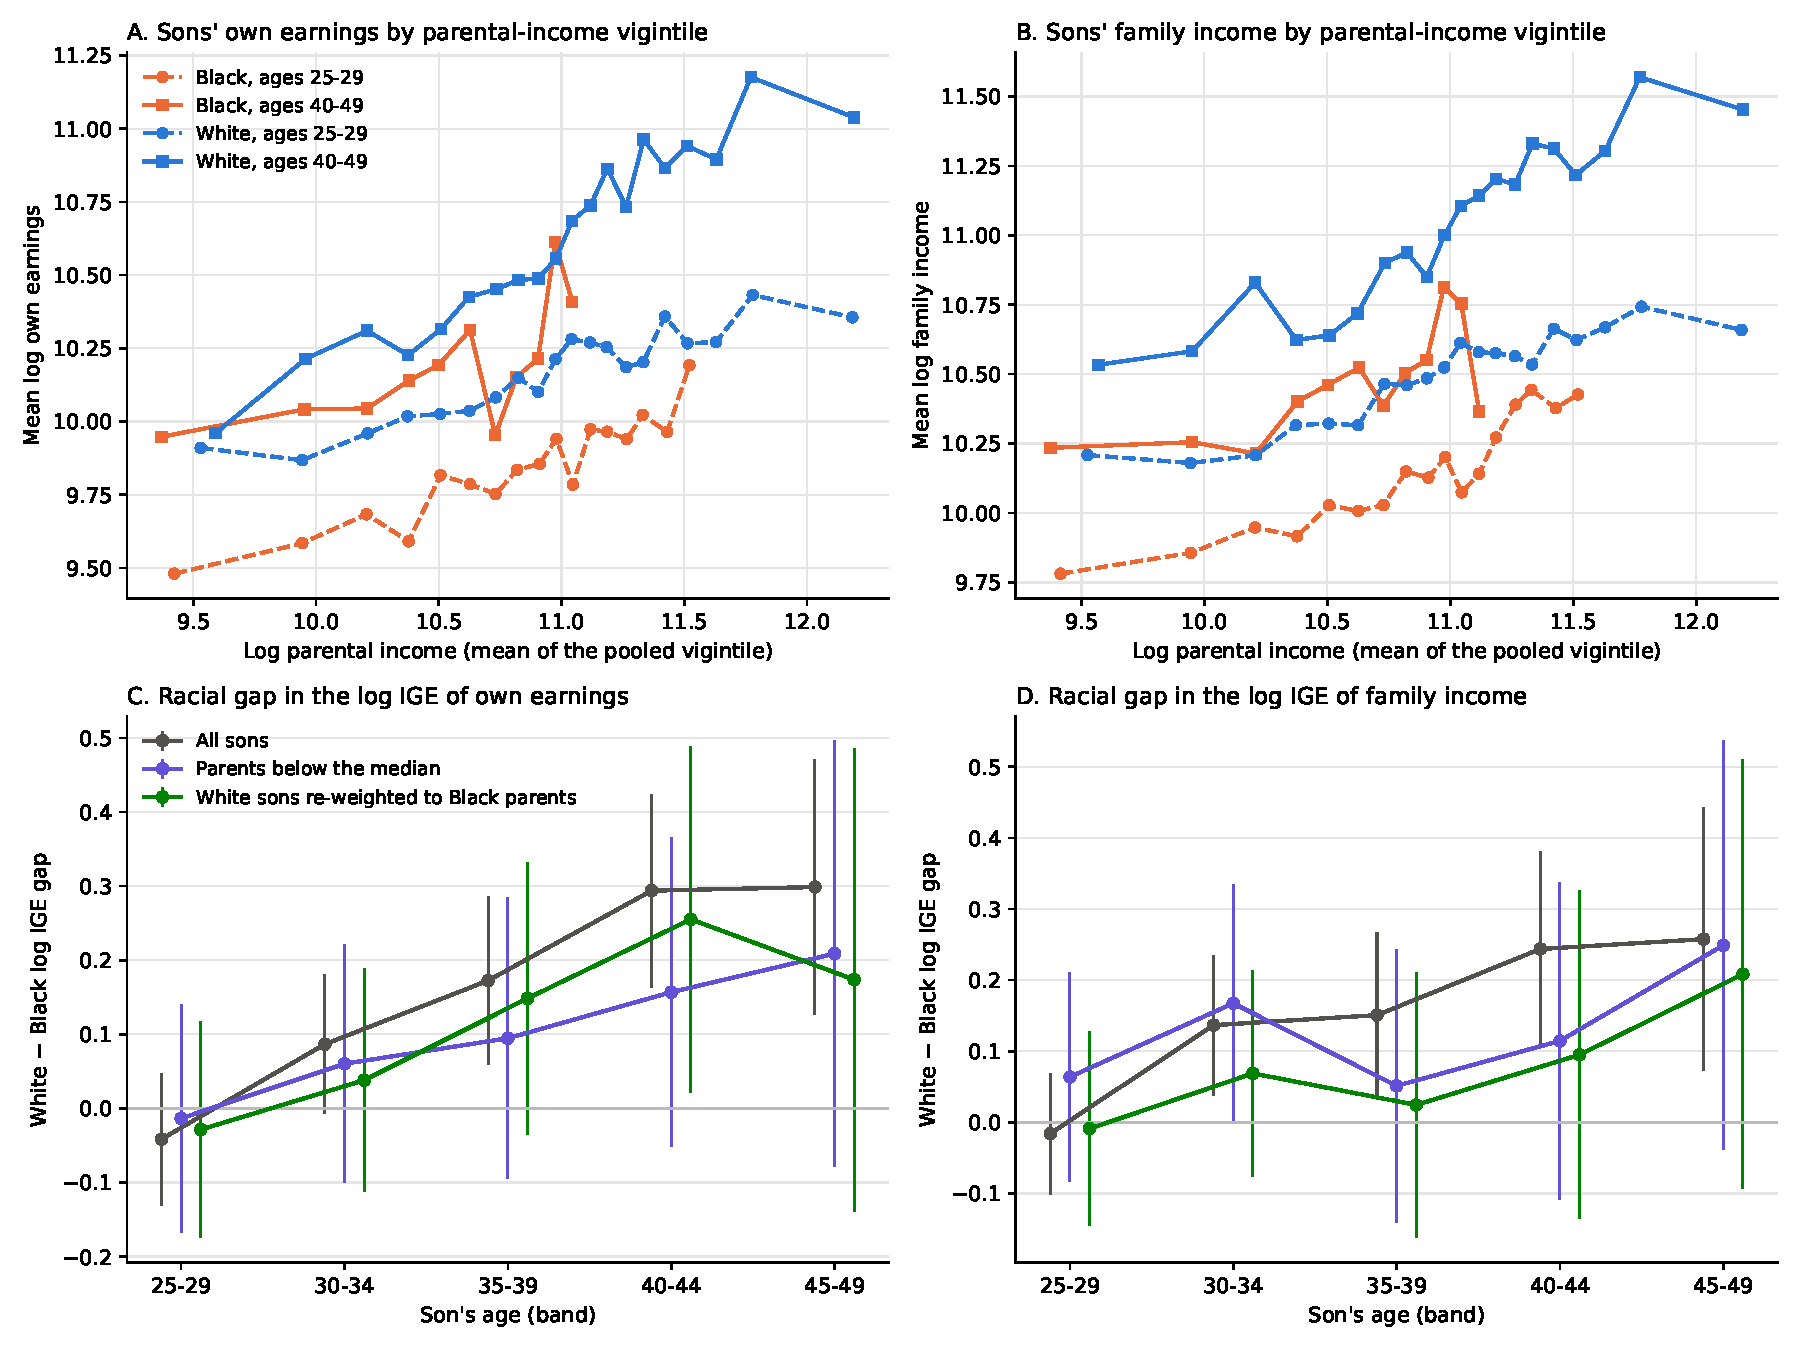
\includegraphics[width=\textwidth]{paperB_position.pdf}
\caption{Race or position in the parental distribution? (PSID, sons)}\label{fig:position}
\begin{minipage}{\textwidth}\footnotesize \textit{Notes:} Panels A and B: mean log outcome (net of race-specific
single-age means) by vigintile of the pooled parental-income distribution of Black and White sons, at 25--29 (dashed)
and 40--49 (solid); vigintiles with at least 20 sons of the race. Panels C and D: White $-$ Black gap in the log IGE by
age band, all sons, sons of parents below the pooled median, and White sons re-weighted to the Black distribution of
parental income in each band (20 bins); 95\% confidence intervals clustered by 1968 family. Code:
\texttt{41.AgeProfileMeasurement.py} and \texttt{44.PaperBReviewTables.py}.\end{minipage}
\end{figure}

\paragraph{Daughters.} Daughters' family income shows the same divergence (gap trend 0.162$^{***}$, s.e.\ 0.032),
their own earnings do not (Appendix Table~\ref{tab:ige_daughters}). The daughters' divergence runs through their
husbands (Section~\ref{sec:contains}), and it rests on the low-income oversample: on the SRC sample alone it is 0.014
(0.106).\footnote{\texttt{output/age\_profile\_robustness.md}, Section 3. Code: \texttt{33.AgeProfileRobustness.py}.}


\subsection{What opens: wages, not hours, shocks or marriage}\label{sec:contains}

Family income at a given age is the product of a household's composition, its members' hours and their wages, and it
is hit by transitory shocks. Each could produce a racial gap in persistence that opens with age. This subsection tests
them in turn. The analyses that need the father's own wage and hours use father-present sons
(Section~\ref{sec:data}); everything here is accounting, not a causal decomposition.

\paragraph{Wages, not hours.} Log earnings are the sum of the log hourly wage and log annual hours, so the elasticity of
sons' earnings with respect to fathers' earnings splits exactly into a part carried by the son's wage and a part
carried by his hours. In the age-interacted design at 40 the earnings elasticity is 0.220 for Black and 0.389 for
White sons, and the son's wage carries 0.210 and 0.378 of it, his hours 0.010 and 0.012 (Appendix
Table~\ref{tab:pricequantity}). The wage is also where the gap opens (Table~\ref{tab:wageage}). At 25--34 the elasticity
of sons' earnings with respect to fathers' earnings is 0.259 for Black and 0.258 for White sons (White $-$ Black
$-0.002$, s.e.\ 0.050), and at 35--44 it is 0.260 and 0.384 (0.123$^{*}$, s.e.\ 0.070). The gradient of the son's log
wage in parental income rises from 0.255 at 25--34 to 0.403 at 35--44 for White sons and stays at 0.161--0.163 for
Black sons, so the White $-$ Black gap in it grows from 0.094$^{***}$ to 0.240$^{***}$. The hours gradient is larger for
Black sons at 25--34 (White $-$ Black $-0.058^{***}$), so hours raise the Black elasticity and partly hide the wage gap
at young ages.\footnote{The PSID wage is annual earnings over annual hours, so the split could inherit division bias if
hours were measured with more error for Black sons; the NLSY79 hourly rate of pay gives the same direction
(Section~\ref{sec:careers}). Code: \texttt{24.IGEDecomposition.py}, Sections 1 and 1c.}

\begin{table}[!htbp]
\centering
\caption{Where the racial gap opens: wage and hours persistence by the son's age (PSID)}
\label{tab:wageage}
\resizebox{\ifdim\width>\textwidth\textwidth\else\width\fi}{!}{%
\resizebox*{!}{\ifdim\totalheight>0.85\textheight 0.85\textheight\else\totalheight\fi}{%
\begin{tabular}{lcccccc}
\toprule
Panel / group & \begin{tabular}[b]{@{}c@{}}ln family income\\on ln parental\\income\end{tabular} & \begin{tabular}[b]{@{}c@{}}ln wage\\on ln parental\\income\end{tabular} & \begin{tabular}[b]{@{}c@{}}ln hours\\on ln parental\\income\end{tabular} & \begin{tabular}[b]{@{}c@{}}ln earnings\\on father's\\ln earnings\end{tabular} & \begin{tabular}[b]{@{}c@{}}ln wage\\on father's\\ln wage\end{tabular} & \begin{tabular}[b]{@{}c@{}}ln hours\\on father's\\ln hours\end{tabular} \\
 & (1) & (2) & (3) & (4) & (5) & (6) \\
\midrule
\multicolumn{7}{l}{\textit{Sons aged 25--34}} \\
Black & $0.273^{***}$ & $0.161^{***}$ & $0.086^{***}$ & $0.259^{***}$ & $0.187^{***}$ & $0.153^{***}$ \\
 & (0.033) & (0.020) & (0.015) & (0.044) & (0.040) & (0.051) \\
White & $0.327^{***}$ & $0.255^{***}$ & $0.027^{**}$ & $0.258^{***}$ & $0.274^{***}$ & $0.131^{***}$ \\
 & (0.026) & (0.020) & (0.012) & (0.024) & (0.022) & (0.028) \\
White $-$ Black & $0.054$ & $0.094^{***}$ & $-0.058^{***}$ & $-0.002$ & $0.086^{*}$ & $-0.022$ \\
 & (0.042) & (0.028) & (0.019) & (0.050) & (0.046) & (0.058) \\
Child-years (Black / White) & 9,226 / 15,304 & 8,331 / 14,761 & 8,331 / 14,761 & 3,995 / 12,399 & 3,995 / 12,399 & 3,995 / 12,399 \\
\addlinespace
\multicolumn{7}{l}{\textit{Sons aged 35--44}} \\
Black & $0.288^{***}$ & $0.163^{***}$ & $0.059^{***}$ & $0.260^{***}$ & $0.207^{***}$ & $0.143^{***}$ \\
 & (0.046) & (0.028) & (0.017) & (0.062) & (0.054) & (0.056) \\
White & $0.474^{***}$ & $0.403^{***}$ & $0.043^{***}$ & $0.384^{***}$ & $0.393^{***}$ & $0.073^{**}$ \\
 & (0.036) & (0.031) & (0.013) & (0.033) & (0.036) & (0.031) \\
White $-$ Black & $0.186^{***}$ & $0.240^{***}$ & $-0.016$ & $0.123^{*}$ & $0.186^{***}$ & $-0.071$ \\
 & (0.058) & (0.042) & (0.022) & (0.070) & (0.065) & (0.064) \\
Child-years (Black / White) & 5,102 / 9,435 & 4,469 / 8,851 & 4,469 / 8,851 & 2,344 / 7,574 & 2,344 / 7,574 & 2,344 / 7,574 \\
\addlinespace
\multicolumn{7}{l}{\textit{Sons aged 45--55}} \\
Black & $0.250^{***}$ & $0.161^{***}$ & $0.045^{*}$ & $0.212^{**}$ & $0.162^{**}$ & $0.052$ \\
 & (0.075) & (0.045) & (0.024) & (0.089) & (0.074) & (0.073) \\
White & $0.474^{***}$ & $0.454^{***}$ & $-0.014$ & $0.403^{***}$ & $0.425^{***}$ & $0.069$ \\
 & (0.060) & (0.047) & (0.027) & (0.052) & (0.051) & (0.052) \\
White $-$ Black & $0.224^{**}$ & $0.293^{***}$ & $-0.059$ & $0.190^{*}$ & $0.262^{***}$ & $0.017$ \\
 & (0.096) & (0.065) & (0.037) & (0.103) & (0.090) & (0.090) \\
Child-years (Black / White) & 2,271 / 4,385 & 1,873 / 3,953 & 1,873 / 3,953 & 1,002 / 3,423 & 1,002 / 3,423 & 1,002 / 3,423 \\
\addlinespace
\multicolumn{7}{l}{\textit{Sons aged 25--55}} \\
Black & $0.274^{***}$ & $0.162^{***}$ & $0.072^{***}$ & $0.255^{***}$ & $0.191^{***}$ & $0.138^{***}$ \\
 & (0.036) & (0.021) & (0.013) & (0.046) & (0.043) & (0.039) \\
White & $0.391^{***}$ & $0.324^{***}$ & $0.027^{**}$ & $0.315^{***}$ & $0.332^{***}$ & $0.105^{***}$ \\
 & (0.028) & (0.022) & (0.011) & (0.025) & (0.026) & (0.027) \\
White $-$ Black & $0.117^{**}$ & $0.163^{***}$ & $-0.045^{***}$ & $0.060$ & $0.141^{***}$ & $-0.033$ \\
 & (0.046) & (0.031) & (0.017) & (0.052) & (0.050) & (0.048) \\
Child-years (Black / White) & 16,599 / 29,124 & 14,673 / 27,565 & 14,673 / 27,565 & 7,341 / 23,396 & 7,341 / 23,396 & 7,341 / 23,396 \\
\bottomrule
\end{tabular}}}
\par\smallskip
\begin{minipage}{\textwidth}\footnotesize \textit{Notes:} One regression per cell: child-years of sons in the age band of the panel, outcome and regressor in the column header, Lee--Solon controls (quartics in the parent's age at 16 and the son's age) without the age interactions, so each coefficient is the average slope in the band. Columns (1)--(3): all sons, parental family income (mean at 13--19); columns (4)--(6): father-present sons, father's childhood-window means. White $-$ Black standard error = root sum of squared standard errors (disjoint clusters). Unweighted. Standard errors clustered by 1968 family. $^{***}$ $p<0.01$, $^{**}$ $p<0.05$, $^{*}$ $p<0.1$. Source: \texttt{24.IGEDecomposition.py} (\texttt{output/ige\_decomposition.csv}); table built by \texttt{28.PaperBTables.py}.\end{minipage}
\end{table}


\paragraph{Not shocks or instability.} Thirty-seven percent of Black sons' years at 25--55, against 19 percent of White
sons', involve displacement or unemployment. Instability nonetheless does not produce the divergence. Its gradient in
parental income is the same for the two races at every age (equality across bands, $p=0.524$;
Appendix Table~\ref{tab:mechtests}); the earnings gap computed over clean years opens with age exactly as over all years
(0.196$^{***}$ against 0.193$^{***}$); and purging shock years from both generations moves the gap by 0.002 (0.042),
removing reduced-hours years as well by 0.018 (0.044).\footnote{Appendix Tables~\ref{tab:instability} and
\ref{tab:purging}; the hours share of the father's earnings variance, which a noisier father-side measure would
inflate, accounts for about 0.02 of the gap (Table~\ref{tab:decomposition}). Code: \texttt{24.IGEDecomposition.py}.}

\paragraph{Not marriage, for sons; husbands, for daughters.} For sons the family-income and earnings elasticities are
nearly the same in both races (gaps at 40 of 0.204$^{***}$ and 0.244$^{***}$), and own earnings carry the whole
family-income gap and its rise (0.221$^{***}$); being partnered rises equally with parental income for Black and White
sons after 35, and controlling for it leaves the gap unchanged (Appendix Table~\ref{tab:mechtests}). Later marriage of White
sons of richer parents holds down their family income at 25--29, which is one reason the family-income gap starts at
zero. For daughters the divergence is in family income and not in their own earnings (gaps at 40 of 0.162$^{***}$ and
0.035), and the channel is the husband: the elasticity of the husband's earnings is 0.370$^{***}$ for White and
0.171$^{***}$ for Black daughters, and the spouse term accounts for three quarters of the daughters' family-income gap
at 40 and for 0.175$^{***}$ of its rise with age (Appendix Table~\ref{tab:incomechannels}).\footnote{Exact log split of family
income into own earnings, the spouse and other income; standard errors clustered by 1968 family. Assortative mating is
strong: the elasticity of a daughter's husband's earnings, 0.362$^{***}$, exceeds that of her own, 0.301$^{***}$
\citep[as in][]{chadwick2002intergenerational}. The daughters' divergence rests on the SEO sample, as
shown above. Code: \texttt{34.IncomeVsEarningsIGE.py}.} The racial divergence that sons show in
their own wages, daughters show in their husbands'.


\paragraph{Parental income concept.} With parents' combined labor income instead of total family income as the
parental measure, the sons' earnings result holds (an opening of 0.134$^{***}$) while the family-income result weakens
to 0.051 (0.045).\footnote{\texttt{output/age\_profile\_robustness.md}, Section 3; half of the drop is the smaller
sample with parental labor income. Code: \texttt{33.AgeProfileRobustness.py}.} Transfers and other non-labor
income in the parental measure matter for the Black family-income profile.


\subsection{Careers: same-employer growth, schooling and job moves}\label{sec:careers}

Using pairs of consecutive interviews one to two years apart at which the son stayed with the same employer, I regress
the annualised growth of his log wage on parental income (Table~\ref{tab:growthladder}). For White sons at 25--34 the
gradient is 0.021$^{***}$ (0.006): a White son whose parents had twice the income sees his wage grow about 1.4 percentage
points a year faster with the same employer, on mean growth of 5.7 percent. For Black sons it is 0.003 (0.008), and the
racial difference, 0.018$^{*}$ ($p=0.062$), is less precisely estimated than its components. The White gradient is not
measurement: over two intervals it is 0.019$^{***}$ and among strict stayers whose tenure covers both income years
0.013$^{**}$.\footnote{Controlling for the wage at the interview before the pair raises it to 0.036$^{***}$, so it is not
catch-up after a low start; over whole employer spells it is 0.019$^{***}$. \texttt{output/same\_employer\_growth\_checks.md},
Section B. Code: \texttt{36.SameEmployerGrowthChecks.py}.} About half of it is sorting into steep jobs: within the
cell of the first interview of the pair it is 0.011$^{*}$ ($p=0.095$), within the cell of the later interview 0.006
($p=0.34$), and within cells the racial difference is 0.006--0.007, not significant. Controlling for the son's years of
education lowers it to 0.008 ($p=0.17$). In the NLSY79, where the employer is observed directly in the job roster, the
White gradient is 0.008$^{*}$ and the Black gradient zero, and holding the AFQT and education fixed brings the White
gradient to 0.002: the part explained runs through education (0.0046$^{***}$), not measured ability (0.0014, $p=0.31$).
The precise statement is: for White sons the gradient is precisely estimated, half sorting and half growth within jobs,
and mostly schooling; for Black sons it is a precise zero; the racial difference in growth within the same job is not
established.\footnote{Annual growth between two interviews is too noisy to settle the part that does not run through
schooling. Cumulated over ten and twenty years of a son's own wage, the PSID gradient at equal schooling is
0.073$^{***}$ and 0.135$^{***}$ for White sons and about zero for Black sons with the 13--19 mean of parental income,
and about zero with a one-year measure, in the PSID as in the NLSY79 and NLSY97. Code:
\texttt{67.LongDifferenceH4.py}, \texttt{68.LongDifferenceMeasurement.py} and \texttt{69.LongDifferenceNLSY97.py}.}

\begin{table}[!htbp]
\centering
\caption{Wage growth with the same employer at 25--34: parental income, schooling and ability}
\label{tab:growthladder}
\resizebox{\ifdim\width>\textwidth\textwidth\else\width\fi}{!}{%
\resizebox*{!}{\ifdim\totalheight>0.85\textheight 0.85\textheight\else\totalheight\fi}{%
\begin{tabular}{lcccccccccc}
\toprule
 & \begin{tabular}[b]{@{}c@{}}PSID\\baseline\end{tabular} & \begin{tabular}[b]{@{}c@{}}PSID\\cell FE,\\first interview\end{tabular} & \begin{tabular}[b]{@{}c@{}}PSID\\cell FE,\\later interview\end{tabular} & \begin{tabular}[b]{@{}c@{}}PSID\\+ education\end{tabular} & \begin{tabular}[b]{@{}c@{}}PSID\\two-interval\\growth\end{tabular} & \begin{tabular}[b]{@{}c@{}}PSID\\strict\\stayers\end{tabular} & \begin{tabular}[b]{@{}c@{}}NLSY79\\baseline\end{tabular} & \begin{tabular}[b]{@{}c@{}}NLSY79\\+ AFQT\end{tabular} & \begin{tabular}[b]{@{}c@{}}NLSY79\\+ education\end{tabular} & \begin{tabular}[b]{@{}c@{}}NLSY79\\+ AFQT\\+ education\end{tabular} \\
 & (1) & (2) & (3) & (4) & (5) & (6) & (7) & (8) & (9) & (10) \\
\midrule
\multicolumn{11}{l}{\textit{White sons}} \\
Log parental income & $0.021^{***}$ & $0.011^{*}$ & $0.006$ & $0.008$ & $0.019^{***}$ & $0.013^{**}$ & $0.008^{*}$ & $0.004$ & $0.002$ & $0.002$ \\
 & (0.006) & (0.006) & (0.007) & (0.006) & (0.005) & (0.006) & (0.005) & (0.005) & (0.005) & (0.005) \\
Years of education &  &  &  & $0.009^{***}$ &  &  &  &  & $0.004^{***}$ & $0.004^{***}$ \\
 &  &  &  & (0.002) &  &  &  &  & (0.001) & (0.001) \\
AFQT (1 s.d.) &  &  &  &  &  &  &  & $0.009^{***}$ &  & $0.003$ \\
 &  &  &  &  &  &  &  & (0.003) &  & (0.003) \\
\addlinespace
\multicolumn{11}{l}{\textit{Black sons}} \\
Log parental income & $0.003$ & $0.004$ & $-0.001$ & $0.002$ & $-0.001$ & $0.010$ & $0.000$ & $0.000$ & $-0.002$ & $-0.001$ \\
 & (0.008) & (0.010) & (0.009) & (0.008) & (0.007) & (0.008) & (0.005) & (0.005) & (0.005) & (0.005) \\
Years of education &  &  &  & $0.002$ &  &  &  &  & $0.003$ & $0.004$ \\
 &  &  &  & (0.003) &  &  &  &  & (0.002) & (0.002) \\
AFQT (1 s.d.) &  &  &  &  &  &  &  & $0.003$ &  & $-0.003$ \\
 &  &  &  &  &  &  &  & (0.005) &  & (0.005) \\
\addlinespace
\multicolumn{11}{l}{\textit{White $-$ Black}} \\
Log parental income & $0.018^{*}$ & $0.006$ & $0.007$ & $0.006$ & $0.019^{**}$ & $0.003$ & $0.009$ & $0.004$ & $0.004$ & $0.003$ \\
 & (0.010) & (0.012) & (0.011) & (0.010) & (0.008) & (0.010) & (0.007) & (0.007) & (0.007) & (0.007) \\
Years of education &  &  &  & $0.006^{*}$ &  &  &  &  & $0.001$ & $0.000$ \\
 &  &  &  & (0.003) &  &  &  &  & (0.002) & (0.003) \\
AFQT (1 s.d.) &  &  &  &  &  &  &  & $0.006$ &  & $0.006$ \\
 &  &  &  &  &  &  &  & (0.006) &  & (0.006) \\
\bottomrule
\end{tabular}}}
\par\smallskip
\begin{minipage}{\textwidth}\footnotesize \textit{Notes:} Pairs of consecutive interviews one to two years apart at which the son is with the same employer (PSID: tenure covers the interval; NLSY79: the same employer in the job roster), sons aged 25--34 at the later interview. Outcome: annualised growth of the log hourly wage. One regression per column and race; controls in every column: quartic in age, year (round) fixed effects. Cell: 11 occupation groups $\times$ 33 industry groups. Two-interval growth: the same employer at three interviews. Strict stayers: tenure covers both income years. NLSY79 columns: common sample with AFQT and education known; AFQT standardised within birth year. White $-$ Black: difference of the separate regressions, joint influence functions, clustered by 1968 family (PSID) or 1979 household (NLSY79). $^{***}$ $p<0.01$, $^{**}$ $p<0.05$, $^{*}$ $p<0.1$. Source: \texttt{IGE/36.SameEmployerGrowthChecks.py} (\texttt{output/same\_employer\_growth\_checks.csv}).\end{minipage}
\end{table}



If schooling carries the gradient, the distinctive prediction is that its pay-off grows over the career.
\citet{bhuller2017life} show in Norwegian registers that education premiums rise steeply with age.
Table~\ref{tab:schooling} estimates the return to a year of schooling in the PSID by age band and race. For White sons the
return in hourly wages rises from 0.049 at 25--29 to 0.128 at 40--44, and in earnings from 0.045 to 0.143; for Black sons
it starts higher---0.076 in wages and 0.124 in earnings at 25--29---and rises much less in wages and not at all in
earnings (0.12--0.15 at every age). The White--Black difference in the rise is 0.032$^{***}$ (0.011) in wages and
0.055$^{***}$ (0.014) in earnings, and 0.013$^{*}$ (0.008) for the NLSY79 hourly rate of pay. Education accounts for a
large part of the divergence: adding years of schooling to the regression of the log wage on parental income by band
removes 0.057$^{***}$ of the pooled rise of wage persistence after 35 (a share of 0.44$^{***}$), and 0.069$^{***}$ of the
0.186$^{***}$ change in the racial gap (0.37$^{***}$); for earnings 0.090$^{***}$ of 0.203$^{***}$ (0.44$^{***}$), and in
the NLSY79 0.038$^{***}$ of 0.054$^{**}$ (0.72$^{**}$). Education is an outcome of the same background, so these are
shares of accounting, not causal mediation.\footnote{Code: \texttt{42.SchoolingAndJobGrowth.py}
(\texttt{output/schooling\_job\_growth.md}).}


\paragraph{Within jobs, net of the calendar, holding ability fixed.} A steeper White return could reflect access alone:
if good jobs accumulate human capital faster and educated White sons get more of them, the return to schooling rises
faster with age for White sons with no racial difference in what schooling does on a given job. The test holds the job
fixed (Table~\ref{tab:withincell}). On son-years with an early job, the White--Black difference in the rise of the
earnings return is 0.058$^{***}$ (0.014) without cell controls, 0.061$^{***}$ (0.018) with fixed effects for the son's
cell at 25--34 and 0.066$^{***}$ (0.016) with fixed effects for his current cell; in wages 0.031$^{***}$, 0.029$^{*}$ and
0.036$^{***}$. Holding the early job fixed halves the rise of the earnings return in the pooled sample (from 0.050$^{***}$ to
0.025$^{***}$), so half of the rising return is the sorting of the educated into steep jobs; but it lowers the rise for
both races alike, and the racial difference does not move (changes of $-0.002$ to 0.009, s.e.\ 0.011--0.016).
The rise of the college premium over 1980--2000 could make a return rise with age that is really a rise with calendar
time; allowing the return to trend with the calendar leaves the racial difference in the rise at 0.063$^{**}$ (0.027)
for earnings and 0.035 ($p=0.12$) for wages, and within the cohorts born 1955--69 it is 0.051$^{***}$ and 0.029$^{*}$. In
the NLSY79, a single cohort, the difference is 0.017$^{*}$ within the current cell and 0.021$^{**}$ (0.009) when the AFQT
is held fixed. The Black sons' higher return at 25--29 also survives the job (0.061$^{***}$ in earnings within the early
cell) in the PSID, but not in the NLSY79 (0.008).\footnote{Code: \texttt{45.WithinCellIdentification.py}
(\texttt{output/within\_cell\_identification.md}); NLSY79 AFQT results in Appendix Table~\ref{tab:afqtgrowth}.}

The age pattern of the returns says which mechanism this is. Under employer learning the coefficient on schooling, which
employers see, falls with experience, and the coefficient on ability, which they learn, rises
\citep{altonji2001employer, lange2007speed, arcidiacono2010beyond}. In the NLSY79 both rise: with the AFQT and schooling
in the same regression, the schooling coefficient rises by 0.049$^{***}$ from the bands below 35 to the bands above, and
the AFQT coefficient by 0.036$^{***}$, and the AFQT rise does not differ by race ($-0.031$, s.e.\ 0.025). A rising return
to schooling is the complementarity of schooling with human capital accumulated on the job \citep{bhuller2017life},
and it is this complementarity that is weaker for Black sons, within the same job and at equal measured ability.
The return to experience itself does not differ by race at equal AFQT: in the within-decile regression of
\citet{rauh2023black}, run on the NLSY79 with its supplemental Black sample, hourly earnings grow with experience at the
same rate for Black and White men (Black $\times$ experience 0.003 in logs, s.e.\ 0.003, $p = 0.30$; 1,184 Black men).
Their model holds accumulation race-neutral given the AFQT and has no schooling; the racial difference here is in how
growth varies with schooling.\footnote{Hourly earnings (2018 dollars, and logs) on Black, years of accumulated
experience, their product and region fixed effects by AFQT decile, men aged 23--54 not in school, at least 500 hours and
25 weeks in the year; standard errors clustered by person. On the cross-sectional sample (285 Black men) the regression
reproduces their pattern: no difference in deciles 1--5, and negative Black $\times$ experience in deciles 9 and 10
($-1.03^{**}$ and $-1.93^{***}$ dollars a year, $p = 0.034$ and $p < 0.001$), cells that hold 4 and 3 Black men. With
the supplemental sample no decile differs and the slope pooled within deciles is 0.028 dollars a year (s.e.\ 0.071,
$p = 0.70$). Code: \texttt{70.RauhReplication.py}; output \texttt{output/rauh\_replication.md}.}
The same-employer evidence points the same way but is weaker: a year of schooling raises same-employer wage growth at
25--34 by 0.010$^{***}$ for White and 0.003 for Black sons (difference 0.007$^{**}$, $p=0.030$), and within the cell of
the first interview the difference is 0.004 ($p=0.37$); in the NLSY79 it is 0.002 ($p=0.47$) and 0.005$^{*}$ within the
cell.


Wage growth comes from staying, from moving and from losing jobs \citep{topel1992job, altonji2013modeling}.
Table~\ref{tab:jobmoves} splits the parental-income gradient of annual wage growth into these three parts. For White
sons at 25--34 the gradient of 0.020$^{***}$ is almost all within jobs: 0.017$^{***}$ comes from years with the same
employer, 0.001 from moves and 0.003 from displacements. For Black sons the within-job part is 0.005, and moves
contribute $-0.008^{**}$: Black sons of richer parents gain less, not more, when they change employers. Of the racial
difference in the growth gradient at 25--34, 0.021$^{***}$, about three fifths is within jobs (0.012$^{*}$) and two fifths
at moves (0.009$^{**}$); the racial difference in the gain at a move is 0.069$^{**}$ (0.028). Family background buys the
same protection from job loss in both races: the probability of displacement falls with parental income by 0.037$^{***}$
for White and 0.038$^{***}$ for Black sons.

\begin{table}[!htbp]
\centering
\caption{Wage growth within and between jobs by parental income (PSID, sons)}
\label{tab:jobmoves}
\resizebox{\ifdim\width>\textwidth\textwidth\else\width\fi}{!}{%
\resizebox*{!}{\ifdim\totalheight>0.85\textheight 0.85\textheight\else\totalheight\fi}{%
\begin{tabular}{lcccccccc}
\toprule
 & \begin{tabular}[b]{@{}c@{}}Wage growth,\\all pairs\end{tabular} & \begin{tabular}[b]{@{}c@{}}Contribution:\\stayed\end{tabular} & \begin{tabular}[b]{@{}c@{}}Contribution:\\moved\end{tabular} & \begin{tabular}[b]{@{}c@{}}Contribution:\\displaced\end{tabular} & \begin{tabular}[b]{@{}c@{}}Stayed\end{tabular} & \begin{tabular}[b]{@{}c@{}}Displaced\end{tabular} & \begin{tabular}[b]{@{}c@{}}Growth\\if stayed\end{tabular} & \begin{tabular}[b]{@{}c@{}}Growth\\if moved\end{tabular} \\
 & (1) & (2) & (3) & (4) & (5) & (6) & (7) & (8) \\
\midrule
\multicolumn{9}{l}{\textit{Sons aged 25--34}} \\
White: log parental income & $0.020^{***}$ & $0.017^{***}$ & $0.001$ & $0.003$ & $0.035^{***}$ & $-0.037^{***}$ & $0.020^{***}$ & $0.005$ \\
 & (0.005) & (0.004) & (0.002) & (0.002) & (0.012) & (0.009) & (0.006) & (0.017) \\
Black: log parental income & $-0.001$ & $0.005$ & $-0.008^{**}$ & $0.002$ & $0.035^{**}$ & $-0.038^{***}$ & $0.004$ & $-0.064^{***}$ \\
 & (0.006) & (0.005) & (0.003) & (0.004) & (0.016) & (0.014) & (0.008) & (0.023) \\
White $-$ Black: log parental income & $0.021^{***}$ & $0.012^{*}$ & $0.009^{**}$ & $0.000$ & $0.000$ & $0.001$ & $0.016$ & $0.069^{**}$ \\
 & (0.008) & (0.007) & (0.004) & (0.005) & (0.020) & (0.017) & (0.010) & (0.028) \\
\addlinespace
\multicolumn{9}{l}{\textit{Sons aged 35--55}} \\
White: log parental income & $0.007^{**}$ & $0.003$ & $0.004^{**}$ & $0.000$ & $0.033^{***}$ & $-0.021^{**}$ & $0.003$ & $0.046^{***}$ \\
 & (0.003) & (0.003) & (0.002) & (0.001) & (0.011) & (0.008) & (0.004) & (0.017) \\
Black: log parental income & $-0.002$ & $0.000$ & $-0.002$ & $-0.001$ & $-0.005$ & $0.000$ & $0.000$ & $-0.013$ \\
 & (0.004) & (0.003) & (0.002) & (0.003) & (0.015) & (0.011) & (0.004) & (0.020) \\
White $-$ Black: log parental income & $0.009^{*}$ & $0.003$ & $0.006^{**}$ & $0.000$ & $0.039^{**}$ & $-0.021$ & $0.002$ & $0.059^{**}$ \\
 & (0.005) & (0.004) & (0.003) & (0.003) & (0.019) & (0.014) & (0.005) & (0.026) \\
\bottomrule
\end{tabular}}}
\par\smallskip
\begin{minipage}{\textwidth}\footnotesize \textit{Notes:} Consecutive interviews one to two years apart with a valid wage, a mapped occupation and tenure (waves 1985--2023). Between the two wage years the son stayed with the employer, moved without displacement, or was displaced (plant closure, layoff or firing). Columns (2)--(4) are the wage growth times an indicator of the event and add up to column (1) on the same pairs (column (3) and (4) of the moved and displaced contributions); (5)--(6) linear probabilities; (7)--(8) growth conditional on the event. Each cell: coefficient on log parental income; controls: quartic in age, year fixed effects; standard errors clustered by 1968 family. $^{***}$ $p<0.01$, $^{**}$ $p<0.05$, $^{*}$ $p<0.1$. Source: \texttt{IGE/42.SchoolingAndJobGrowth.py} (\texttt{output/schooling\_job\_growth.csv}).\end{minipage}
\end{table}


\subsection{What does not carry the divergence}

Entry into supervisory and managerial occupations, the closest observable analogue to the promotion delays documented
by \citet{hegde2026racial}, rises with parental income after 35 for White and not for Black sons (a racial difference of
0.024$^{***}$ at 35--55), but the change of that difference relative to 25--34 is 0.008 (0.011), and self-reported
position changes and promotions show no Black deficit. Job loss is frequent and costly---displacement lowers the son's log
wage two to three years later by 0.131$^{***}$, of which 0.028$^{***}$ is a lower occupational score---but the
occupational loss is not larger for Black sons, and shocks do not account for the divergence (Section~\ref{sec:contains}).
These results, the industry decompositions and the NLSY79 replication of the occupational split are in
Appendix~\ref{app:careers}.


\subsection{Fathers' jobs}\label{sec:fathers}

Parents' employers and networks shape where young people find their first job and raise their initial earnings
\citep{corak2011intergenerational, kramarz2014strong, staiger2022}. The PSID does not identify employers, and neither
do the public NLSY files for fathers, so working for the father's employer cannot be observed; the father's occupation
group and his occupation-by-industry cell, his modal codes when the son was 12--18, are the proxies.\footnote{The
father is the male head of the son's family at 16, so these measures exist for 52 percent of Black and 87 percent of
White sons. Fathers are coded in 1970 Census codes and sons after 2001 in 2000 or 2010 codes; the 35--55 window falls
more often after 2001, so coding drift lowers measured following after 35, which works against the convergence below.
Code: \texttt{32.IndustryCareers.py}, \texttt{35.EarlyIndustryLatePayoff.py} and
\texttt{43.FatherJobSelfEmployment.py}.}

\paragraph{Following pays at entry, not in growth.} Sons work in their father's industry group two to three times as
often as random matching within race and parental-income tercile would predict (14.2 percent of White sons at 35--55
against a benchmark of 5.1 percent, and 10.1 percent of Black sons against 5.4 percent). Holding the son's education
and the level and slope of his industry fixed, sons in their father's industry group earn 0.079$^{***}$ more at 25--34
and 0.054$^{*}$ more at 35--55, but their wages grow no faster (0.005, s.e.\ 0.005), and following accounts for none of
the racial divergence ($-0.002$ of 0.107$^{**}$).\footnote{Appendix Table~\ref{tab:fatherindustry} and
\texttt{output/industry\_careers.md}, Section 4. Few Black fathers worked in high-paying service industries (21 in
finance, insurance or real estate), so industry-specific following cannot be estimated for Black sons.} Family networks,
as measured here, transmit a starting advantage that is the same at every age at which the IGE is measured.

\paragraph{Convergence on the father's occupation.} Over the career, sons of richer parents converge on their fathers'
occupations (Table~\ref{tab:fatherse}). The parental-income gradient of being in the father's occupation group is
0.051$^{***}$ at 25--34 and 0.099$^{***}$ at 35--55 (change 0.052$^{***}$). The change is precisely estimated for White
sons (0.060$^{***}$) and imprecise for Black sons (0.036, s.e.\ 0.028); the two cannot be distinguished. The level of
following differs by race at every age: at 35--55, 22.4 percent of White and 15.3 percent of Black sons work in their
father's occupation group. Within the top parental tercile, sons of White parents are 11.7 percentage points more likely
than sons of Black parents to work in their father's occupation group (0.117$^{***}$, resting on 121 Black sons in that
tercile), while rich and poor White sons do not differ ($-0.086$, s.e.\ 0.061): the contrast is a racial gap in
following the father's occupation at equal parental income, not class amplifying it.

\paragraph{The father's exact job is a family business.} Whether a son holds his father's exact job---his occupation
group in his industry group---does not depend on parental income at 25--34 (0.004) and does at 35--55 (0.031$^{**}$;
change 0.023$^{**}$), because sons of richer parents who hold it in their early thirties keep it: among the 137 sons in
the father's cell at 25--34, 84 are still in it at 35--55 and 53 leave, and leaving falls with parental income
($-0.206^{***}$); entry after 34 is rare (39 of 1,892 sons) and unrelated to parental income. Only 9 of the 84 who keep
the father's job are Black. The self-employment split shows what the exact job is. Twenty-one percent of White and 8
percent of Black sons have a self-employed father, and the convergence comes entirely from them: among sons of
self-employed fathers the gradient rises by 0.065$^{***}$ after 35, among other sons by 0.009 (0.011), and among sons
for whom neither father nor son is self-employed by 0.005. The cells most often inherited after 35 are farming in
agriculture (31 sons, 56 percent of them self-employed and 75 percent with a self-employed father), craft work in
construction and management in construction. Convergence on the father's exact job is the inheritance of a farm or a
firm \citep[the business and wealth transmission of][]{fagereng2021wealthy}, not of a position in a network. The
occupation-level result is not: excluding self-employed fathers, the gradient still rises after 35 (0.037$^{*}$) and the
rich-White-versus-rich-Black contrast is unchanged (0.117$^{***}$). Keeping the father's job also does not depend on
self-employment ($-0.183^{**}$ among the 90 sons of fathers who were not self-employed), and holding the father's exact
job brings no wage premium at 35--55 and no faster wage growth.

\begin{table}[!htbp]
\centering
\caption{Fathers' jobs and self-employment (PSID, sons)}
\label{tab:fatherse}
\resizebox{\ifdim\width>\textwidth\textwidth\else\width\fi}{!}{%
\resizebox*{!}{\ifdim\totalheight>0.85\textheight 0.85\textheight\else\totalheight\fi}{%
\begin{tabular}{lcccc}
\toprule
 & \begin{tabular}[b]{@{}c@{}}All sons\end{tabular} & \begin{tabular}[b]{@{}c@{}}Father not\\self-employed\end{tabular} & \begin{tabular}[b]{@{}c@{}}Father\\self-employed\end{tabular} & \begin{tabular}[b]{@{}c@{}}Neither father\\nor son\\self-employed\end{tabular} \\
 & (1) & (2) & (3) & (4) \\
\midrule
\multicolumn{5}{l}{\textit{Son in the father's occupation $\times$ industry cell}} \\
All: log parental income, 25--34 & $0.004$ & $-0.006$ & $0.009$ & $-0.005$ \\
 & (0.012) & (0.012) & (0.023) & (0.013) \\
All: log parental income, 35--55 & $0.031^{**}$ & $0.009$ & $0.072^{***}$ & $0.008$ \\
 & (0.016) & (0.016) & (0.025) & (0.018) \\
All: log parental income $\times$ (age $\geq$ 35) & $0.023^{**}$ & $0.009$ & $0.065^{***}$ & $0.005$ \\
 & (0.010) & (0.011) & (0.021) & (0.012) \\
White: log parental income, 25--34 & $-0.005$ & $-0.011$ & $-0.005$ & $-0.007$ \\
 & (0.014) & (0.014) & (0.025) & (0.015) \\
White: log parental income, 35--55 & $0.025$ & $0.006$ & $0.065^{**}$ & $0.006$ \\
 & (0.020) & (0.020) & (0.025) & (0.023) \\
White: log parental income $\times$ (age $\geq$ 35) & $0.026^{**}$ & $0.009$ & $0.073^{***}$ & $0.004$ \\
 & (0.012) & (0.012) & (0.022) & (0.015) \\
Son-years / sons at 35--55 & 13,835 / 2,166 & 10,539 / 1,683 & 2,399 / 373 & 9,324 / 1,579 \\
\addlinespace
\multicolumn{5}{l}{\textit{Son in the father's occupation group}} \\
All: log parental income, 25--34 & $0.051^{***}$ & $0.040^{**}$ & $0.067^{**}$ & $0.037^{*}$ \\
 & (0.016) & (0.019) & (0.030) & (0.019) \\
All: log parental income, 35--55 & $0.099^{***}$ & $0.071^{***}$ & $0.163^{***}$ & $0.072^{***}$ \\
 & (0.020) & (0.026) & (0.027) & (0.027) \\
All: log parental income $\times$ (age $\geq$ 35) & $0.052^{***}$ & $0.037^{*}$ & $0.104^{***}$ & $0.038^{*}$ \\
 & (0.016) & (0.021) & (0.026) & (0.022) \\
White: log parental income, 25--34 & $0.040^{**}$ & $0.035$ & $0.042$ & $0.033$ \\
 & (0.018) & (0.022) & (0.032) & (0.022) \\
White: log parental income, 35--55 & $0.099^{***}$ & $0.073^{**}$ & $0.161^{***}$ & $0.076^{**}$ \\
 & (0.023) & (0.029) & (0.027) & (0.029) \\
White: log parental income $\times$ (age $\geq$ 35) & $0.060^{***}$ & $0.039^{*}$ & $0.124^{***}$ & $0.041^{*}$ \\
 & (0.017) & (0.022) & (0.028) & (0.024) \\
Son-years / sons at 35--55 & 13,908 / 2,174 & 10,604 / 1,691 & 2,404 / 373 & 9,383 / 1,588 \\
\addlinespace
\multicolumn{5}{l}{\textit{Race, class and keeping the father's job}} \\
Rich White $-$ rich Black, father's occupation group, 35--55 & $0.117^{***}$ & $0.117^{***}$ & $-0.019$ & $0.113^{***}$ \\
 & (0.038) & (0.040) & (0.143) & (0.043) \\
Rich White $-$ rich Black, father's cell, 35--55 & $0.011$ & $-0.008$ & $0.131^{***}$ & $-0.004$ \\
 & (0.029) & (0.030) & (0.033) & (0.033) \\
Black sons in the top tercile & 121 & 112 & 9 & 105 \\
Leaving the father's cell (in at 25--34) on log parental income & $-0.206^{***}$ & $-0.183^{**}$ & $-0.223^{*}$ & $-0.163^{**}$ \\
 & (0.066) & (0.080) & (0.126) & (0.079) \\
Sons in the father's cell at 25--34 & 137 & 90 & 46 & 82 \\
\bottomrule
\end{tabular}}}
\par\smallskip
\begin{minipage}{\textwidth}\footnotesize \textit{Notes:} Son-year linear probability models, Lee--Solon controls (quartics in the parent's age and the son's age), clusters 1968 family; all sons weighted, White sons unweighted. The father's cell is his modal 11 occupation groups $\times$ 33 industry groups when the son is 12--18; the father is self-employed when at least half of his valid interviews from 1976 on, with the son aged 10--25, report working for himself (alone or also for someone else). The change row is from one regression on 25--55 with log parental income $\times$ (age $\geq$ 35). Rich White $-$ rich Black: sons in the top pooled tercile of parental income, race $\times$ tercile cells with log parental income, weighted. Leaving: sons in the father's cell in their modal 25--34 job, out of it in their modal 35--55 job, on log parental income and a quadratic in birth cohort. These estimates use sons with a father's self-employment code (and, for leaving, a cohort quadratic and no weights); on all sons with a father's cell the same contrasts are 0.131$^{***}$ (0.038) for rich White $-$ rich Black and $-0.167^{**}$ (0.067) for leaving (	exttt{35.EarlyIndustryLatePayoff.py}, Section F). $^{***}$ $p<0.01$, $^{**}$ $p<0.05$, $^{*}$ $p<0.1$. Source: \texttt{43.FatherJobSelfEmployment.py} (\texttt{output/father\_job\_selfemp.csv}).\end{minipage}
\end{table}


The fathers' evidence adds two channels to the career evidence: a level advantage at entry through family networks,
which accounts for $-0.002$ (0.004) of the 0.107$^{**}$ change in the racial gap in wage persistence on the father-present
sample, and the inheritance of family businesses, a matter of assets rather than access, which accounts for $-0.004$ of a
0.120$^{**}$ change. Convergence on fathers' occupations outside the family firm, with its racial gap at equal parental
income, is a third. None of them carries the growth of wages that produces the divergence; that is the job at 25--34,
its access, and schooling.
